\documentclass[11pt,a4paper]{article}

\usepackage[headsep=1cm,headheight=3cm,left=3.5cm,right=3.5cm,top=2.5cm,bottom=2.5cm,a4paper]{geometry}

\linespread{1.3}
\setlength{\parindent}{0pt}
\setlength{\parskip}{1em}

\usepackage[spanish]{babel}
\usepackage[utf8]{inputenc}

%% Fuentes personalizadas para utilizar con XeTeX
\usepackage[sfdefault]{roboto}
\usepackage[scaled=0.9]{DejaVuSansMono}
\usepackage[T1]{fontenc}

\usepackage{enumitem}
\setlist[itemize]{leftmargin=*}
\setlist[enumerate]{leftmargin=*}

\usepackage{changepage}

\newcounter{ActCounter}
\newcommand{\act}[1]{\addtocounter{ActCounter}{1}\textbf{\sffamily ACT-\theActCounter}\quad#1\\}

\usepackage{tabularx}
\usepackage{float}
\usepackage{adjustbox}

\title{Práctica 2: Modelo de casos de uso \large\\ Fundamentos de Ingeniería del Software}
\author{Sofía Almedia Bruno \and José Antonio Álvarez Ocete \and Miguel Lentisco Ballesteros \and Simón López Vico \and José María Martín Luque}

\begin{document}

\maketitle

\section{Introducción}

En el presente documento se muestra el modelo de Casos de Uso obtenido en el proceso de análisis del sistema para la gestión de un centro médico. El modelo se puede descomponer en dos grandes paquetes que agrupan las funcionalidades básicas del sistema.

\section{Diagramas de casos de uso} % (fold)

\begin{figure}[H]
	\caption{Diagrama de casos de uso de gestión de datos}
	\centering
	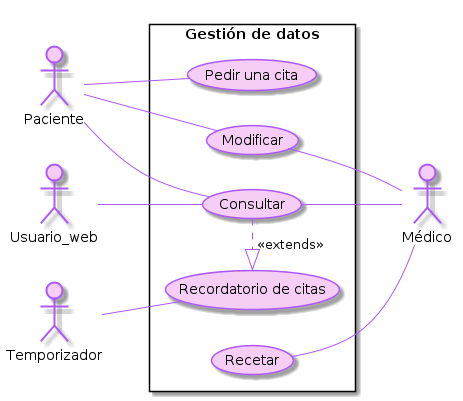
\includegraphics{diagramas/gestion_datos}
\end{figure}

\begin{figure}[H]
	\caption{Diagrama de casos de uso de contabilidad}
	\centering
	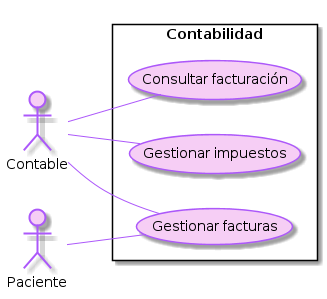
\includegraphics{diagramas/contabilidad}
\end{figure}

\section{Descripción de los actores}
% PLANTILLA PACIENTE

\begin{table}[H]
\label{my-label}
\begin{tabularx}{\textwidth}{l|Xlllr}
	\textbf{Actor}           & \multicolumn{4}{l}{Paciente} & \act\\ 
	\textbf{Descripción}     & \multicolumn{5}{>{\hsize=2\hsize}X}{Paciente adscrito al centro médico que desea pedir cita, consultar su historial o informarse acerca de la clínica}\\
	\textbf{Características} & \multicolumn{5}{>{\hsize=2\hsize}X}{Todos los clientes de la clínica son pacientes}\\ 
	\textbf{Relaciones}      & \multicolumn{5}{>{\hsize=2\hsize}X}{}\\ 
	\textbf{Referencias}     & \multicolumn{5}{>{\hsize=2\hsize}X}{}\\
	\textbf{Autor}           &  & \textbf{Fecha} &  & \textbf{Versión} & \textbf{}                      \\ 
\end{tabularx}
\end{table}

\vspace{1cm}

\begin{table}[H]
\label{my-label}
\begin{tabularx}{\textwidth}{lXl}
	\textbf{Atributos} &  & \\
	\textbf{Nombre}    & \textbf{Descripción} & \textbf{Tipo} \\ \hline
	Datos personales   & Identifican al paciente (\texttt{Id\_paciente}, DNI, nombre y apellidos, ...)     & \\
	Contacto           & Permiten ponerse en contacto con el paciente o algún familiar (teléfono, en caso de emergencia avisar a ...) & \\  
	Datos médicos      & Información relativa a la salud del paciente (historial médico, grupo sanguíneo, enfermedades previas, alergias, ...)            
\end{tabularx}
\end{table}

\vspace{1cm}

\begin{table}[H]
\begin{tabularx}{\textwidth}{lXX}
	\textbf{Comentarios} &  &  \\ \hline
\end{tabularx}
\end{table}
% FIN PLANTILLA PACIENTE

\vspace{2cm}

% PLANTILLA MÉDICO

\begin{table}[H]
\label{my-label}
\begin{tabularx}{\textwidth}{l|Xlllr}
	\textbf{Actor}           & Médico & & & & \act \\ 
	\textbf{Descripción}     & \multicolumn{5}{>{\hsize=2\hsize}X}{Personal sanitario de la clínica}\\
	\textbf{Características} & \multicolumn{5}{>{\hsize=2\hsize}X}{Puede modificar la información del paciente}\\ 
	\textbf{Relaciones}      & \multicolumn{5}{>{\hsize=2\hsize}X}{}\\ 
	\textbf{Referencias}     & \multicolumn{5}{>{\hsize=2\hsize}X}{}\\ 
	\textbf{Autor}           &  & \textbf{Fecha} & & \textbf{Versión} & \\ 
\end{tabularx}
\end{table}

\vspace{1cm}

\begin{table}[H]
\label{my-label}
\begin{tabularx}{\textwidth}{lXl}
	\textbf{Atributos} &  & \\
	\textbf{Nombre}    & \textbf{Descripción} & \textbf{Tipo} \\ \hline
	Datos personales   &  Identifican al médico (\texttt{Id\_médico}, DNI, nombre y apellidos,...)     & \\
	Datos laborales    & Relativos a su trabajo (horario, sueldo, vacaciones,...) &
\end{tabularx}
\end{table}

\vspace{1cm}

\begin{table}[H]
\begin{tabularx}{\textwidth}{lXX}
	\textbf{Comentarios} &  &  \\ \hline
\end{tabularx}
\end{table}

% FIN PLANTILLA MÉDICO

\vspace{2cm}

% PLANTILLA CONTABLE

\begin{table}[H]
	\label{my-label}
	\begin{tabularx}{\textwidth}{l|Xlllr}
		\textbf{Actor}           & \multicolumn{4}{l}{Contable} & \act\\ 
		\textbf{Descripción}     & \multicolumn{5}{>{\hsize=2\hsize}X}{Encargado de gestionar la facturación y los impuestos referentes a la clínica.}\\
		\textbf{Características} & \multicolumn{5}{>{\hsize=2\hsize}X}{Puede consultar las facturas de todo cliente en el sistema y el sueldo del personal, así como etiquetar como moroso a aquel cliente que debe dinero.}\\ 
		\textbf{Relaciones}      & \multicolumn{5}{>{\hsize=2\hsize}X}{Paciente, personal.}\\ 
		\textbf{Referencias}     & \multicolumn{5}{>{\hsize=2\hsize}X}{Consultar facturación, gestionar impuestos, gestionar facturas.}\\
		\textbf{Autor}           & Simón López & \textbf{Fecha} & 04/04/18 & \textbf{Versión} & \textbf{1.0}                      \\ 
	\end{tabularx}
\end{table}

\vspace{1cm}

\begin{table}[H]
	\label{my-label}
	\begin{tabularx}{\textwidth}{lXl}
		\textbf{Atributos}  &  & \\
		\textbf{Nombre}     & \textbf{Descripción} & \textbf{Tipo} \\ \hline
		\textbf{IdContable} & Nombre o pseudónimo referente al contable, único en el sistema que identificará a este. & Texto \\
		\textbf{Salario}    & Cantidad de dinero que cobra el contable al mes. & Numérico \\
	\end{tabularx}
\end{table}

\vspace{1cm}

\begin{table}[H]
	\begin{tabularx}{\textwidth}{lXX}
		\textbf{Comentarios} &  &  \\ \hline
		Usualmente no habrá más de un contable por clínica.
	\end{tabularx}
\end{table}

%FIN DE LA PLANTILLA CONTABLE

% PLANTILLA USUARIO WEB

\begin{table}[H]
	\label{my-label}
	\begin{tabularx}{\textwidth}{l|Xlllr}
		\textbf{Actor}           & \multicolumn{4}{l}{Usuario web} & \act\\ 
		\textbf{Descripción}     & \multicolumn{5}{>{\hsize=2\hsize}X}{Cualquier persona que acceda a la información disponible en la página web}\\
		\textbf{Características} & \multicolumn{5}{>{\hsize=2\hsize}X}{Puede acceder a diversa información tal como las especialidades, tratamientos, horarios, instalaciones o médicos disponibles.}\\ 
		\textbf{Relaciones}      & \multicolumn{5}{>{\hsize=2\hsize}X}{No tiene.}\\ 
		\textbf{Referencias}     & \multicolumn{5}{>{\hsize=2\hsize}X}{}\\
		\textbf{Autor}           & Miguel Lentisco & \textbf{Fecha} & 04/04/18 & \textbf{Versión} & \textbf{1.0}                      \\ 
	\end{tabularx}
\end{table}

\vspace{1cm}

\begin{table}[H]
	\begin{tabularx}{\textwidth}{lXX}
		\textbf{Comentarios} &  &  \\ \hline
		No se va a guardar información sobre estos usuarios, puede ser cualquier persona que quiera informarse sobre la clínica.
	\end{tabularx}
\end{table}





% FIN DE LA PLANTILLA USUARIO WEB


\section{Descripción de los casos de uso}

% Usar la plantilla general

\section{Diagrama de paquetes}

	
\end{document}
